% Options for packages loaded elsewhere
\PassOptionsToPackage{unicode}{hyperref}
\PassOptionsToPackage{hyphens}{url}
\PassOptionsToPackage{dvipsnames,svgnames,x11names}{xcolor}
%
\documentclass[
  12pt,
]{article}

\usepackage{amsmath,amssymb}
\usepackage{setspace}
\usepackage{iftex}
\ifPDFTeX
  \usepackage[T1]{fontenc}
  \usepackage[utf8]{inputenc}
  \usepackage{textcomp} % provide euro and other symbols
\else % if luatex or xetex
  \usepackage{unicode-math}
  \defaultfontfeatures{Scale=MatchLowercase}
  \defaultfontfeatures[\rmfamily]{Ligatures=TeX,Scale=1}
\fi
\usepackage{lmodern}
\ifPDFTeX\else  
    % xetex/luatex font selection
  \setmainfont[]{Times New Roman}
\fi
% Use upquote if available, for straight quotes in verbatim environments
\IfFileExists{upquote.sty}{\usepackage{upquote}}{}
\IfFileExists{microtype.sty}{% use microtype if available
  \usepackage[]{microtype}
  \UseMicrotypeSet[protrusion]{basicmath} % disable protrusion for tt fonts
}{}
\makeatletter
\@ifundefined{KOMAClassName}{% if non-KOMA class
  \IfFileExists{parskip.sty}{%
    \usepackage{parskip}
  }{% else
    \setlength{\parindent}{0pt}
    \setlength{\parskip}{6pt plus 2pt minus 1pt}}
}{% if KOMA class
  \KOMAoptions{parskip=half}}
\makeatother
\usepackage{xcolor}
\usepackage[margin=2cm]{geometry}
\setlength{\emergencystretch}{3em} % prevent overfull lines
\setcounter{secnumdepth}{5}
% Make \paragraph and \subparagraph free-standing
\ifx\paragraph\undefined\else
  \let\oldparagraph\paragraph
  \renewcommand{\paragraph}[1]{\oldparagraph{#1}\mbox{}}
\fi
\ifx\subparagraph\undefined\else
  \let\oldsubparagraph\subparagraph
  \renewcommand{\subparagraph}[1]{\oldsubparagraph{#1}\mbox{}}
\fi

\usepackage{color}
\usepackage{fancyvrb}
\newcommand{\VerbBar}{|}
\newcommand{\VERB}{\Verb[commandchars=\\\{\}]}
\DefineVerbatimEnvironment{Highlighting}{Verbatim}{commandchars=\\\{\}}
% Add ',fontsize=\small' for more characters per line
\usepackage{framed}
\definecolor{shadecolor}{RGB}{241,243,245}
\newenvironment{Shaded}{\begin{snugshade}}{\end{snugshade}}
\newcommand{\AlertTok}[1]{\textcolor[rgb]{0.68,0.00,0.00}{#1}}
\newcommand{\AnnotationTok}[1]{\textcolor[rgb]{0.37,0.37,0.37}{#1}}
\newcommand{\AttributeTok}[1]{\textcolor[rgb]{0.40,0.45,0.13}{#1}}
\newcommand{\BaseNTok}[1]{\textcolor[rgb]{0.68,0.00,0.00}{#1}}
\newcommand{\BuiltInTok}[1]{\textcolor[rgb]{0.00,0.23,0.31}{#1}}
\newcommand{\CharTok}[1]{\textcolor[rgb]{0.13,0.47,0.30}{#1}}
\newcommand{\CommentTok}[1]{\textcolor[rgb]{0.37,0.37,0.37}{#1}}
\newcommand{\CommentVarTok}[1]{\textcolor[rgb]{0.37,0.37,0.37}{\textit{#1}}}
\newcommand{\ConstantTok}[1]{\textcolor[rgb]{0.56,0.35,0.01}{#1}}
\newcommand{\ControlFlowTok}[1]{\textcolor[rgb]{0.00,0.23,0.31}{#1}}
\newcommand{\DataTypeTok}[1]{\textcolor[rgb]{0.68,0.00,0.00}{#1}}
\newcommand{\DecValTok}[1]{\textcolor[rgb]{0.68,0.00,0.00}{#1}}
\newcommand{\DocumentationTok}[1]{\textcolor[rgb]{0.37,0.37,0.37}{\textit{#1}}}
\newcommand{\ErrorTok}[1]{\textcolor[rgb]{0.68,0.00,0.00}{#1}}
\newcommand{\ExtensionTok}[1]{\textcolor[rgb]{0.00,0.23,0.31}{#1}}
\newcommand{\FloatTok}[1]{\textcolor[rgb]{0.68,0.00,0.00}{#1}}
\newcommand{\FunctionTok}[1]{\textcolor[rgb]{0.28,0.35,0.67}{#1}}
\newcommand{\ImportTok}[1]{\textcolor[rgb]{0.00,0.46,0.62}{#1}}
\newcommand{\InformationTok}[1]{\textcolor[rgb]{0.37,0.37,0.37}{#1}}
\newcommand{\KeywordTok}[1]{\textcolor[rgb]{0.00,0.23,0.31}{#1}}
\newcommand{\NormalTok}[1]{\textcolor[rgb]{0.00,0.23,0.31}{#1}}
\newcommand{\OperatorTok}[1]{\textcolor[rgb]{0.37,0.37,0.37}{#1}}
\newcommand{\OtherTok}[1]{\textcolor[rgb]{0.00,0.23,0.31}{#1}}
\newcommand{\PreprocessorTok}[1]{\textcolor[rgb]{0.68,0.00,0.00}{#1}}
\newcommand{\RegionMarkerTok}[1]{\textcolor[rgb]{0.00,0.23,0.31}{#1}}
\newcommand{\SpecialCharTok}[1]{\textcolor[rgb]{0.37,0.37,0.37}{#1}}
\newcommand{\SpecialStringTok}[1]{\textcolor[rgb]{0.13,0.47,0.30}{#1}}
\newcommand{\StringTok}[1]{\textcolor[rgb]{0.13,0.47,0.30}{#1}}
\newcommand{\VariableTok}[1]{\textcolor[rgb]{0.07,0.07,0.07}{#1}}
\newcommand{\VerbatimStringTok}[1]{\textcolor[rgb]{0.13,0.47,0.30}{#1}}
\newcommand{\WarningTok}[1]{\textcolor[rgb]{0.37,0.37,0.37}{\textit{#1}}}

\providecommand{\tightlist}{%
  \setlength{\itemsep}{0pt}\setlength{\parskip}{0pt}}\usepackage{longtable,booktabs,array}
\usepackage{calc} % for calculating minipage widths
% Correct order of tables after \paragraph or \subparagraph
\usepackage{etoolbox}
\makeatletter
\patchcmd\longtable{\par}{\if@noskipsec\mbox{}\fi\par}{}{}
\makeatother
% Allow footnotes in longtable head/foot
\IfFileExists{footnotehyper.sty}{\usepackage{footnotehyper}}{\usepackage{footnote}}
\makesavenoteenv{longtable}
\usepackage{graphicx}
\makeatletter
\def\maxwidth{\ifdim\Gin@nat@width>\linewidth\linewidth\else\Gin@nat@width\fi}
\def\maxheight{\ifdim\Gin@nat@height>\textheight\textheight\else\Gin@nat@height\fi}
\makeatother
% Scale images if necessary, so that they will not overflow the page
% margins by default, and it is still possible to overwrite the defaults
% using explicit options in \includegraphics[width, height, ...]{}
\setkeys{Gin}{width=\maxwidth,height=\maxheight,keepaspectratio}
% Set default figure placement to htbp
\makeatletter
\def\fps@figure{htbp}
\makeatother
% definitions for citeproc citations
\NewDocumentCommand\citeproctext{}{}
\NewDocumentCommand\citeproc{mm}{%
  \begingroup\def\citeproctext{#2}\cite{#1}\endgroup}
\makeatletter
 % allow citations to break across lines
 \let\@cite@ofmt\@firstofone
 % avoid brackets around text for \cite:
 \def\@biblabel#1{}
 \def\@cite#1#2{{#1\if@tempswa , #2\fi}}
\makeatother
\newlength{\cslhangindent}
\setlength{\cslhangindent}{1.5em}
\newlength{\csllabelwidth}
\setlength{\csllabelwidth}{3em}
\newenvironment{CSLReferences}[2] % #1 hanging-indent, #2 entry-spacing
 {\begin{list}{}{%
  \setlength{\itemindent}{0pt}
  \setlength{\leftmargin}{0pt}
  \setlength{\parsep}{0pt}
  % turn on hanging indent if param 1 is 1
  \ifodd #1
   \setlength{\leftmargin}{\cslhangindent}
   \setlength{\itemindent}{-1\cslhangindent}
  \fi
  % set entry spacing
  \setlength{\itemsep}{#2\baselineskip}}}
 {\end{list}}
\usepackage{calc}
\newcommand{\CSLBlock}[1]{\hfill\break\parbox[t]{\linewidth}{\strut\ignorespaces#1\strut}}
\newcommand{\CSLLeftMargin}[1]{\parbox[t]{\csllabelwidth}{\strut#1\strut}}
\newcommand{\CSLRightInline}[1]{\parbox[t]{\linewidth - \csllabelwidth}{\strut#1\strut}}
\newcommand{\CSLIndent}[1]{\hspace{\cslhangindent}#1}

\usepackage{booktabs}
\usepackage{longtable}
\usepackage{array}
\usepackage{multirow}
\usepackage{wrapfig}
\usepackage{float}
\usepackage{colortbl}
\usepackage{pdflscape}
\usepackage{tabu}
\usepackage{threeparttable}
\usepackage{threeparttablex}
\usepackage[normalem]{ulem}
\usepackage{makecell}
\usepackage{xcolor}
\usepackage[noblocks]{authblk}
\renewcommand*{\Authsep}{, }
\renewcommand*{\Authand}{, }
\renewcommand*{\Authands}{, }
\renewcommand\Affilfont{\small}
\makeatletter
\@ifpackageloaded{caption}{}{\usepackage{caption}}
\AtBeginDocument{%
\ifdefined\contentsname
  \renewcommand*\contentsname{Table of contents}
\else
  \newcommand\contentsname{Table of contents}
\fi
\ifdefined\listfigurename
  \renewcommand*\listfigurename{List of Figures}
\else
  \newcommand\listfigurename{List of Figures}
\fi
\ifdefined\listtablename
  \renewcommand*\listtablename{List of Tables}
\else
  \newcommand\listtablename{List of Tables}
\fi
\ifdefined\figurename
  \renewcommand*\figurename{Figure}
\else
  \newcommand\figurename{Figure}
\fi
\ifdefined\tablename
  \renewcommand*\tablename{Table}
\else
  \newcommand\tablename{Table}
\fi
}
\@ifpackageloaded{float}{}{\usepackage{float}}
\floatstyle{ruled}
\@ifundefined{c@chapter}{\newfloat{codelisting}{h}{lop}}{\newfloat{codelisting}{h}{lop}[chapter]}
\floatname{codelisting}{Listing}
\newcommand*\listoflistings{\listof{codelisting}{List of Listings}}
\makeatother
\makeatletter
\makeatother
\makeatletter
\@ifpackageloaded{caption}{}{\usepackage{caption}}
\@ifpackageloaded{subcaption}{}{\usepackage{subcaption}}
\makeatother
\ifLuaTeX
  \usepackage{selnolig}  % disable illegal ligatures
\fi
\usepackage{bookmark}

\IfFileExists{xurl.sty}{\usepackage{xurl}}{} % add URL line breaks if available
\urlstyle{same} % disable monospaced font for URLs
\hypersetup{
  pdftitle={Medición de percepciones y preferencias sobre meritocracia en etapa escolar en Chile},
  pdfauthor={Andreas Laffert Tamayo; Tomas Úrzua},
  colorlinks=true,
  linkcolor={blue},
  filecolor={Maroon},
  citecolor={Blue},
  urlcolor={Blue},
  pdfcreator={LaTeX via pandoc}}

\title{Medición de percepciones y preferencias sobre meritocracia en
etapa escolar en Chile}


  \author{Andreas Laffert Tamayo}
            \affil{%
                  Instituto de Sociología, Pontificia Universidad
                  Católica de Chile
              }
        \author{Tomas Úrzua}
            \affil{%
                  Departamento de Sociología, Universidad de Chile
              }
      
\date{}
\begin{document}
\maketitle

\setstretch{1.15}
\section{Introducción}\label{introducciuxf3n}

La creencia de que las desigualdades económicas se justifican por
diferencias en elementos meritocráticos---como el esfuerzo individual y
el talento (\citeproc{ref-young_rise_1958}{Young, 1958})---ha sido
identificada como un mecanismo clave para explicar la persistencia de
las desigualdades. Desde sus inicios, las instituciones educativas han
sido fundamentales en la promoción de estos valores, debido a su
conexión con las promesas de movilidad social y mejores oportunidades de
vida (\citeproc{ref-dubet_repensar_2011}{Dubet, 2011}). Investigaciones
previas muestran que las personas que adhieren con mayor fuerza a
creencias meritocráticas tienden a percibir menos desigualdad,
atribuyendo las diferencias económicas al logro personal más que a
factores estructurales (\citeproc{ref-mijs_paradox_2019}{Mijs, 2019};
\citeproc{ref-wilson_role_2003a}{Wilson, 2003}). A nivel escolar, estas
creencias también legitiman una mayor desigualdad, ya que fomentan
actitudes que aceptan las jerarquías sociales como justas
(\citeproc{ref-batruch_belief_2022}{Batruch et al., 2022};
\citeproc{ref-wiederkehr_belief_2015}{Wiederkehr et al., 2015}). Sin
embargo, los conceptos e instrumentos para medir la meritocracia varían
sustancialmente en la literatura. En respuesta a este problema, Castillo
et al. (\citeproc{ref-castillo_multidimensional_2023}{2023}) proponen un
marco conceptual y de medición para evaluar percepciones y preferencias
meritocráticas y no meritocráticas, demostrando que su escala capta
eficazmente estos constructos en la población adulta chilena.

Con el objetivo de contribuir a la investigación empírica sobre la
formación de la meritocracia y sus factores asociados en edades
tempranas (\citeproc{ref-batruch_belief_2022}{Batruch et al., 2022};
\citeproc{ref-darnon_where_2018}{Darnon et al., 2018};
\citeproc{ref-wiederkehr_belief_2015}{Wiederkehr et al., 2015}), este
estudio busca evaluar la aplicabilidad de dicha escala en la población
escolar de Chile, un país caracterizado por una aguda y persistente
desigualdad económica y un sistema educativo altamente estratificado
(\citeproc{ref-chancel_world_2022}{Chancel et al., 2022};
\citeproc{ref-corvalan_mercado_2017}{Corvalán et al., 2017}). En primer
lugar, argumentamos que existe una distinción entre percepción y
preferencias en meritocracia. Mientras la percepción se asocia con cómo
los individuos ven el funcionamiento de los principios meritocráticos en
la sociedad (lo que es), las preferencias se refieren a juicios
normativos (lo que debería ser). La segunda distinción concierne a
elementos meritocráticos y no meritocráticos. En este caso, también se
considera que aspectos como el rol de los contactos personales y la
riqueza familiar no se oponen necesariamente a la percepción y
valoración del esfuerzo y el talento en la obtención de éxito y
recompensas.

Para determinar hasta qué punto es posible reconocer las distintas
dimensiones de la meritocracia en la población escolar, se implementará
un procedimiento de análisis factorial confirmatorio utilizando datos de
estudiantes chilenos. Además, se estimará la invarianza longitudinal a
través de dos olas de datos de la misma cohorte para evaluar la
estabilidad de la escala en el tiempo.

\section{Datos, Variables y Métodos}\label{datos-variables-y-muxe9todos}

\subsection{Datos}\label{datos}

Este estudio se basa en información proveniente de la base de datos de
la Encuesta Panel sobre Educación y Meritocracia (EDUMER) para sus olas
de 2023 y 2024 en estudiantes. Esta encuesta se basa en la aplicación de
cuestionarios web a estudiantes de sexto básico y primero medio de nueve
colegios de las regiones Metropolitana y de Valparaíso en Chile. La
primera ola incluyó a 846 estudiantes (383 niñas, 418 niños, 45
identificándose como otro; \(M_{edad}\) = 13.1, \(DE_{edad}\) = 1.6), y
la segunda ola siguió a 662 de ellos (302 niñas, 337 niños, 22
identificándose como otro; \(M_{edad}\) = 14.1, \(DE_{edad}\) = 1.6). La
recolección de datos fue financiada por la Agencia Nacional de
Investigación y Desarrollo (ANID) de Chile, bajo el proyecto FONDECYT
N.º 1210847, ``Meritocracia en la escuela: fundamentos morales del
mercado educativo y sus implicancias para la formación ciudadana en
Chile''.

\subsection{Variables}\label{variables}

\textbf{Escala de Percepciones y Preferencias sobre Meritocracia}: Las
variables incluidas en el modelo de medición sobre percepciones y
preferencias meritocráticas y no meritocráticas se operacionalizan según
los mismos ítems propuestos por Castillo et al.
(\citeproc{ref-castillo_multidimensional_2023}{2023}). Esta es una
escala basada en dos componentes, cuatro dimensiones y ocho ítems (dos
por cada dimensión). La percepción de la meritocracia se mide con dos
ítems que indagan el grado de acuerdo con la afirmación de que el
esfuerzo y la habilidad son recompensados en Chile, mientras que la
percepción no meritocrática se mide con dos ítems que evalúan el grado
de acuerdo con la idea de que el éxito está vinculado a los contactos
personales y a la riqueza familiar. La preferencia por la meritocracia
se mide con dos ítems que evalúan el acuerdo con la idea de que quienes
se esfuerzan más o poseen más talento deberían recibir mayores
recompensas. La preferencia por aspectos no meritocráticos se mide con
dos indicadores que evalúan el acuerdo con la idea de que es aceptable
que quienes tienen mejores contactos o padres adinerados tengan más
éxito (ver Table~\ref{tbl-merit}). Cada ítem fue respondido en una
escala Likert de cuatro puntos que va desde ``muy en desacuerdo'' (1)
hasta ``muy de acuerdo'' (4).

\begin{longtable}[]{@{}
  >{\raggedright\arraybackslash}p{(\columnwidth - 4\tabcolsep) * \real{0.0945}}
  >{\raggedright\arraybackslash}p{(\columnwidth - 4\tabcolsep) * \real{0.1339}}
  >{\raggedright\arraybackslash}p{(\columnwidth - 4\tabcolsep) * \real{0.7717}}@{}}

\caption{\label{tbl-merit}Ítems Meritocráticos y No Meritocráticos}

\tabularnewline

\toprule\noalign{}
\begin{minipage}[b]{\linewidth}\raggedright
Componente
\end{minipage} & \begin{minipage}[b]{\linewidth}\raggedright
Dimensión
\end{minipage} & \begin{minipage}[b]{\linewidth}\raggedright
Ítem
\end{minipage} \\
\midrule\noalign{}
\endhead
\bottomrule\noalign{}
\endlastfoot
Percepción & Meritocrática & En Chile, las personas son recompensadas
por su esfuerzo. \\
& Meritocrática & En Chile, las personas son recompensadas por su
inteligencia y habilidades. \\
& No meritocrática & En Chile, a quienes tienen padres ricos les va
mucho mejor en la vida. \\
& No meritocrática & En Chile, a quienes tienen buenos contactos les va
mejor en la vida. \\
Preferencia & Meritocrática & Quienes se esfuerzan más deberían recibir
mayores recompensas que quienes se esfuerzan menos. \\
& Meritocrática & Quienes tienen más talento deberían recibir mayores
recompensas que quienes tienen menos talento. \\
& No meritocrática & Está bien que a quienes tienen padres ricos les
vaya bien en la vida. \\
& No meritocrática & Está bien que a quienes tienen buenos contactos les
vaya bien en la vida. \\

\end{longtable}

\subsection{Métodos}\label{muxe9todos}

Para evaluar nuestras hipótesis, se emplearon análisis factoriales
exploratorios (EFA) y confirmatorios (CFA) basados en un modelo latente
de medición de cuatro factores
(\citeproc{ref-castillo_multidimensional_2023}{Castillo et al., 2023}),
con estimador de Mínimos Cuadrados Ponderados Diagonales (DWLS) debido a
la naturaleza ordinal de los ítems
(\citeproc{ref-kline_principles_2023}{Kline, 2023}). El ajuste del
modelo se evaluó con base en los criterios propuestos por Brown
(\citeproc{ref-brown_confirmatory_2015}{2015}): CFI \textgreater{} 0.95;
TLI \textgreater{} 0.95; RMSEA \textless{} 0.06.

Para examinar la estabilidad métrica del modelo de medición
(\citeproc{ref-davidov_measurement_2014}{Davidov et al., 2014}), se
realizaron pruebas de invarianza longitudinal utilizando los datos de
las dos olas del estudio. En línea con Liu et al.
(\citeproc{ref-liu_testing_2017}{2017}), se siguió un enfoque jerárquico
con cuatro modelos: configural (estructura factorial equivalente), débil
(igualdad de cargas factoriales), fuerte (igualdad de interceptos) y
estricto (igualdad de varianzas de error). Este enfoque es especialmente
relevante para indicadores categóricos ordenados, ya que tratar escalas
Likert de cuatro puntos como continuas puede introducir sesgos en las
estimaciones. Además del criterio de cambio en el chi-cuadrado, se
adoptaron el cambio en CFI (\(\Delta \geq -0.010\)) y en RMSEA
(\(\Delta \geq 0.015\)) como indicadores de invarianza, siguiendo las
recomendaciones de Chen (\citeproc{ref-chen_sensitivity_2007}{2007}).

\section{Resultados}\label{resultados}

\subsection{Descriptivos}\label{descriptivos}

En la Figure~\ref{fig-likert} se presenta la distribución de las
respuestas para los ítems de la escala, organizadas según sus
respectivas dimensiones: percepciones y preferencias. En primer lugar,
en el eje de las percepciones, se observa una alta concentración de
respuestas en las categorías ``de acuerdo'' y ``muy de acuerdo'' para
todos los ítems, lo que indica una fuerte percepción de que los
elementos evaluados influyen efectivamente en el éxito social. Esta
tendencia es particularmente marcada en el ítem referido a los
contactos, seguido por el talento, y con una notable cantidad de
respuestas en ``muy de acuerdo'' respecto al ítem padres ricos. Sin
embargo, también se evidencia cierto grado de disenso: un 33,1\%
considera que el esfuerzo no es recompensado en la sociedad; un 28,6\%
no está de acuerdo con que tener padres ricos implique una ventaja; y un
26,6\% manifiesta desacuerdo respecto a la influencia del talento. El
menor nivel de desacuerdo se registra en el ítem de contactos.

En segundo lugar, en el eje de las preferencias, el patrón se invierte
parcialmente. En el caso del esfuerzo, se observa una fuerte preferencia
por que sea un criterio de recompensa, lo que contrasta con la
percepción sobre su reconocimiento efectivo. En relación con el talento,
un 54,6\% manifiesta preferir que sea recompensado, frente a un 45,4\%
que no lo prefiere. En cuanto a los elementos no meritocráticos, como el
origen familiar, la opinión se encuentra más dividida: en el caso de
padres ricos, las respuestas se reparten casi equitativamente entre
quienes prefieren y quienes no prefieren que este factor influya en el
éxito. Finalmente, respecto a los contactos, se identifica una mayor
proporción de respuestas que expresan preferencia por este criterio.

\begin{figure}

\caption{\label{fig-likert}Distribución de respuestas en los ítems de
Escala de Meritocracia}

\centering{

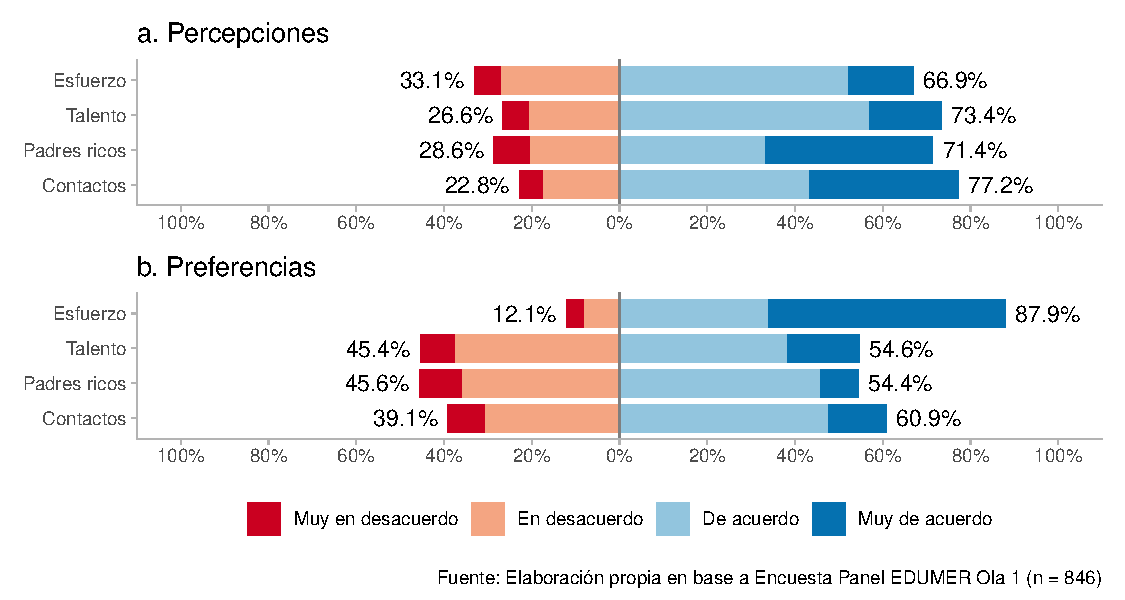
\includegraphics{entrega1_files/figure-pdf/fig-likert-1.pdf}

}

\end{figure}%

En la Table~\ref{tbl-correlaciones} se presenta la matriz de
correlaciones para los items de la escala. En términos generales, se
observa una correlación positiva y de magnitud moderada entre los ítems
que conforman una misma dimensión de la escala. Es decir, los ítems que
miden percepción de esfuerzo y talento (\(r\) = 0.52,
\(p\)\textless.05), así como los que miden percepción sobre padres ricos
y contactos (\(r\) = 0.61, \(p\)\textless.05), tienden a correlacionarse
entre sí. Este patrón también se reproduce en el caso de las
preferencias normativas, donde los ítems dentro de cada subdimensión
presentan correlaciones consistentes entre ellos.

No obstante, un hallazgo relevante es la presencia de correlaciones
positivas, aunque de magnitud débil a moderada, entre ítems que
pertenecen a dimensiones conceptualmente opuestas. Por ejemplo, se
observa que la percepción sobre la influencia de los padres ricos---un
elemento típicamente considerado no meritocrático---se asocia
positivamente con la preferencia por el esfuerzo---un criterio
meritocrático (\(r\) = 0.21). Este mismo patrón se observa con la
percepción sobre el uso de contactos, que también presenta una
correlación positiva con la preferencia por el esfuerzo (\(r\) = 0.26).

En resumen, los datos sugieren que la percepción de que operan
mecanismos no meritocráticos en la sociedad no excluye la preferencia
normativa por criterios meritocráticos. En otras palabras, ambas
lógicas---la meritocrática y la no meritocrática---parecen coexistir en
las creencias de las y los encuestados.

\begin{longtable}[]{@{}
  >{\raggedright\arraybackslash}p{(\columnwidth - 16\tabcolsep) * \real{0.3836}}
  >{\raggedright\arraybackslash}p{(\columnwidth - 16\tabcolsep) * \real{0.0959}}
  >{\raggedright\arraybackslash}p{(\columnwidth - 16\tabcolsep) * \real{0.0959}}
  >{\raggedright\arraybackslash}p{(\columnwidth - 16\tabcolsep) * \real{0.0822}}
  >{\raggedright\arraybackslash}p{(\columnwidth - 16\tabcolsep) * \real{0.0685}}
  >{\raggedright\arraybackslash}p{(\columnwidth - 16\tabcolsep) * \real{0.0822}}
  >{\raggedright\arraybackslash}p{(\columnwidth - 16\tabcolsep) * \real{0.0685}}
  >{\raggedright\arraybackslash}p{(\columnwidth - 16\tabcolsep) * \real{0.0685}}
  >{\raggedright\arraybackslash}p{(\columnwidth - 16\tabcolsep) * \real{0.0548}}@{}}

\caption{\label{tbl-correlaciones}Matriz de correlaciones policóricas
entre los ítems de Escala de Meritocracia}

\tabularnewline

\toprule\noalign{}
\begin{minipage}[b]{\linewidth}\raggedright
\end{minipage} & \begin{minipage}[b]{\linewidth}\raggedright
(A)
\end{minipage} & \begin{minipage}[b]{\linewidth}\raggedright
(B)
\end{minipage} & \begin{minipage}[b]{\linewidth}\raggedright
(C)
\end{minipage} & \begin{minipage}[b]{\linewidth}\raggedright
(D)
\end{minipage} & \begin{minipage}[b]{\linewidth}\raggedright
(E)
\end{minipage} & \begin{minipage}[b]{\linewidth}\raggedright
(F)
\end{minipage} & \begin{minipage}[b]{\linewidth}\raggedright
(G)
\end{minipage} & \begin{minipage}[b]{\linewidth}\raggedright
(H)
\end{minipage} \\
\midrule\noalign{}
\endhead
\bottomrule\noalign{}
\endlastfoot
A. Percepción Esfuerzo & & & & & & & & \\
B. Percepción Talento & 0.52* & & & & & & & \\
C. Percepción Padres Ricos & -0.16 & -0.04. & & & & & & \\
D. Percepción Contactos & -0.10* & 0.01* & 0.61* & & & & & \\
E. Preferencia Esfuerzo & 0.01 & 0.12 & 0.21 & 0.26 & & & & \\
F. Preferencia Talento & -0.04 & 0.08 & 0.16 & 0.25 & 0.36* & & & \\
G. Preferencia Padres Ricos & 0.06 & 0.10 & 0.15 & 0.19 & 0.05 & 0.10 &
& \\
H. Preferencia Contactos & 0.11 & 0.09 & 0.06 & 0.26 & 0.06 & 0.12 &
0.61 & \\

\end{longtable}

\textbf{Note:} \^{}\^{} **p\textless0.01, *p\textless0.5

\subsection{Multivariados}\label{multivariados}

\subsubsection{Análisis factorial
exploratorio}\label{anuxe1lisis-factorial-exploratorio}

\subsubsection{Análisis factorial
confirmatorio}\label{anuxe1lisis-factorial-confirmatorio}

En la Figure~\ref{fig-cfa1} se presenta la solución estandarizada del
modelo factorial confirmatorio estimado para la escala de meritocracia
en la primera ola del estudio. De acuerdo con los grados de libertad, el
modelo se encuentra sobre identidicado (\(df\) = 14 \textgreater{} 0).
Los indicadores de ajuste global muestran que el modelo presenta un buen
ajuste a los datos empíricos. Si bien la prueba del estadístico
\(\chi^2\), que evalúa si existen discrepancias significativas entre la
matriz de covarianza observada y la que es estimada por el modelo
resulta significativa (p \textless{} 0.001), lo cual podría indicar un
mal ajuste del modelo, este resultado debe interpretarse con cautela. Es
bien sabido que esta prueba es altamente sensible al tamaño muestral, y
en muestras superiores a los 200 casos tiende a rechazar la hipótesis
nula incluso ante desviaciones triviales del modelo
(\citeproc{ref-brown_confirmatory_2015}{Brown, 2015}). Por esta razón,
se recurre a indicadores alternativos que son más robustos en este
contexto. En efecto, tanto el índice de ajuste comparativo (CFI) como el
índice de Tucker-Lewis (TLI) y el error cuadrático medio de aproximación
(RMSEA) se encuentran dentro de los umbrales comúnmente aceptados para
indicar un buen ajuste (CFI y TLI \textgreater{} 0.95; RMSEA \textless{}
0.05), lo cual respalda la validez factorial del instrumento.

\begin{figure}

\caption{\label{fig-cfa1}Análisis factorial confirmatorio de Escala de
Meritocracia Ola 1}

\centering{

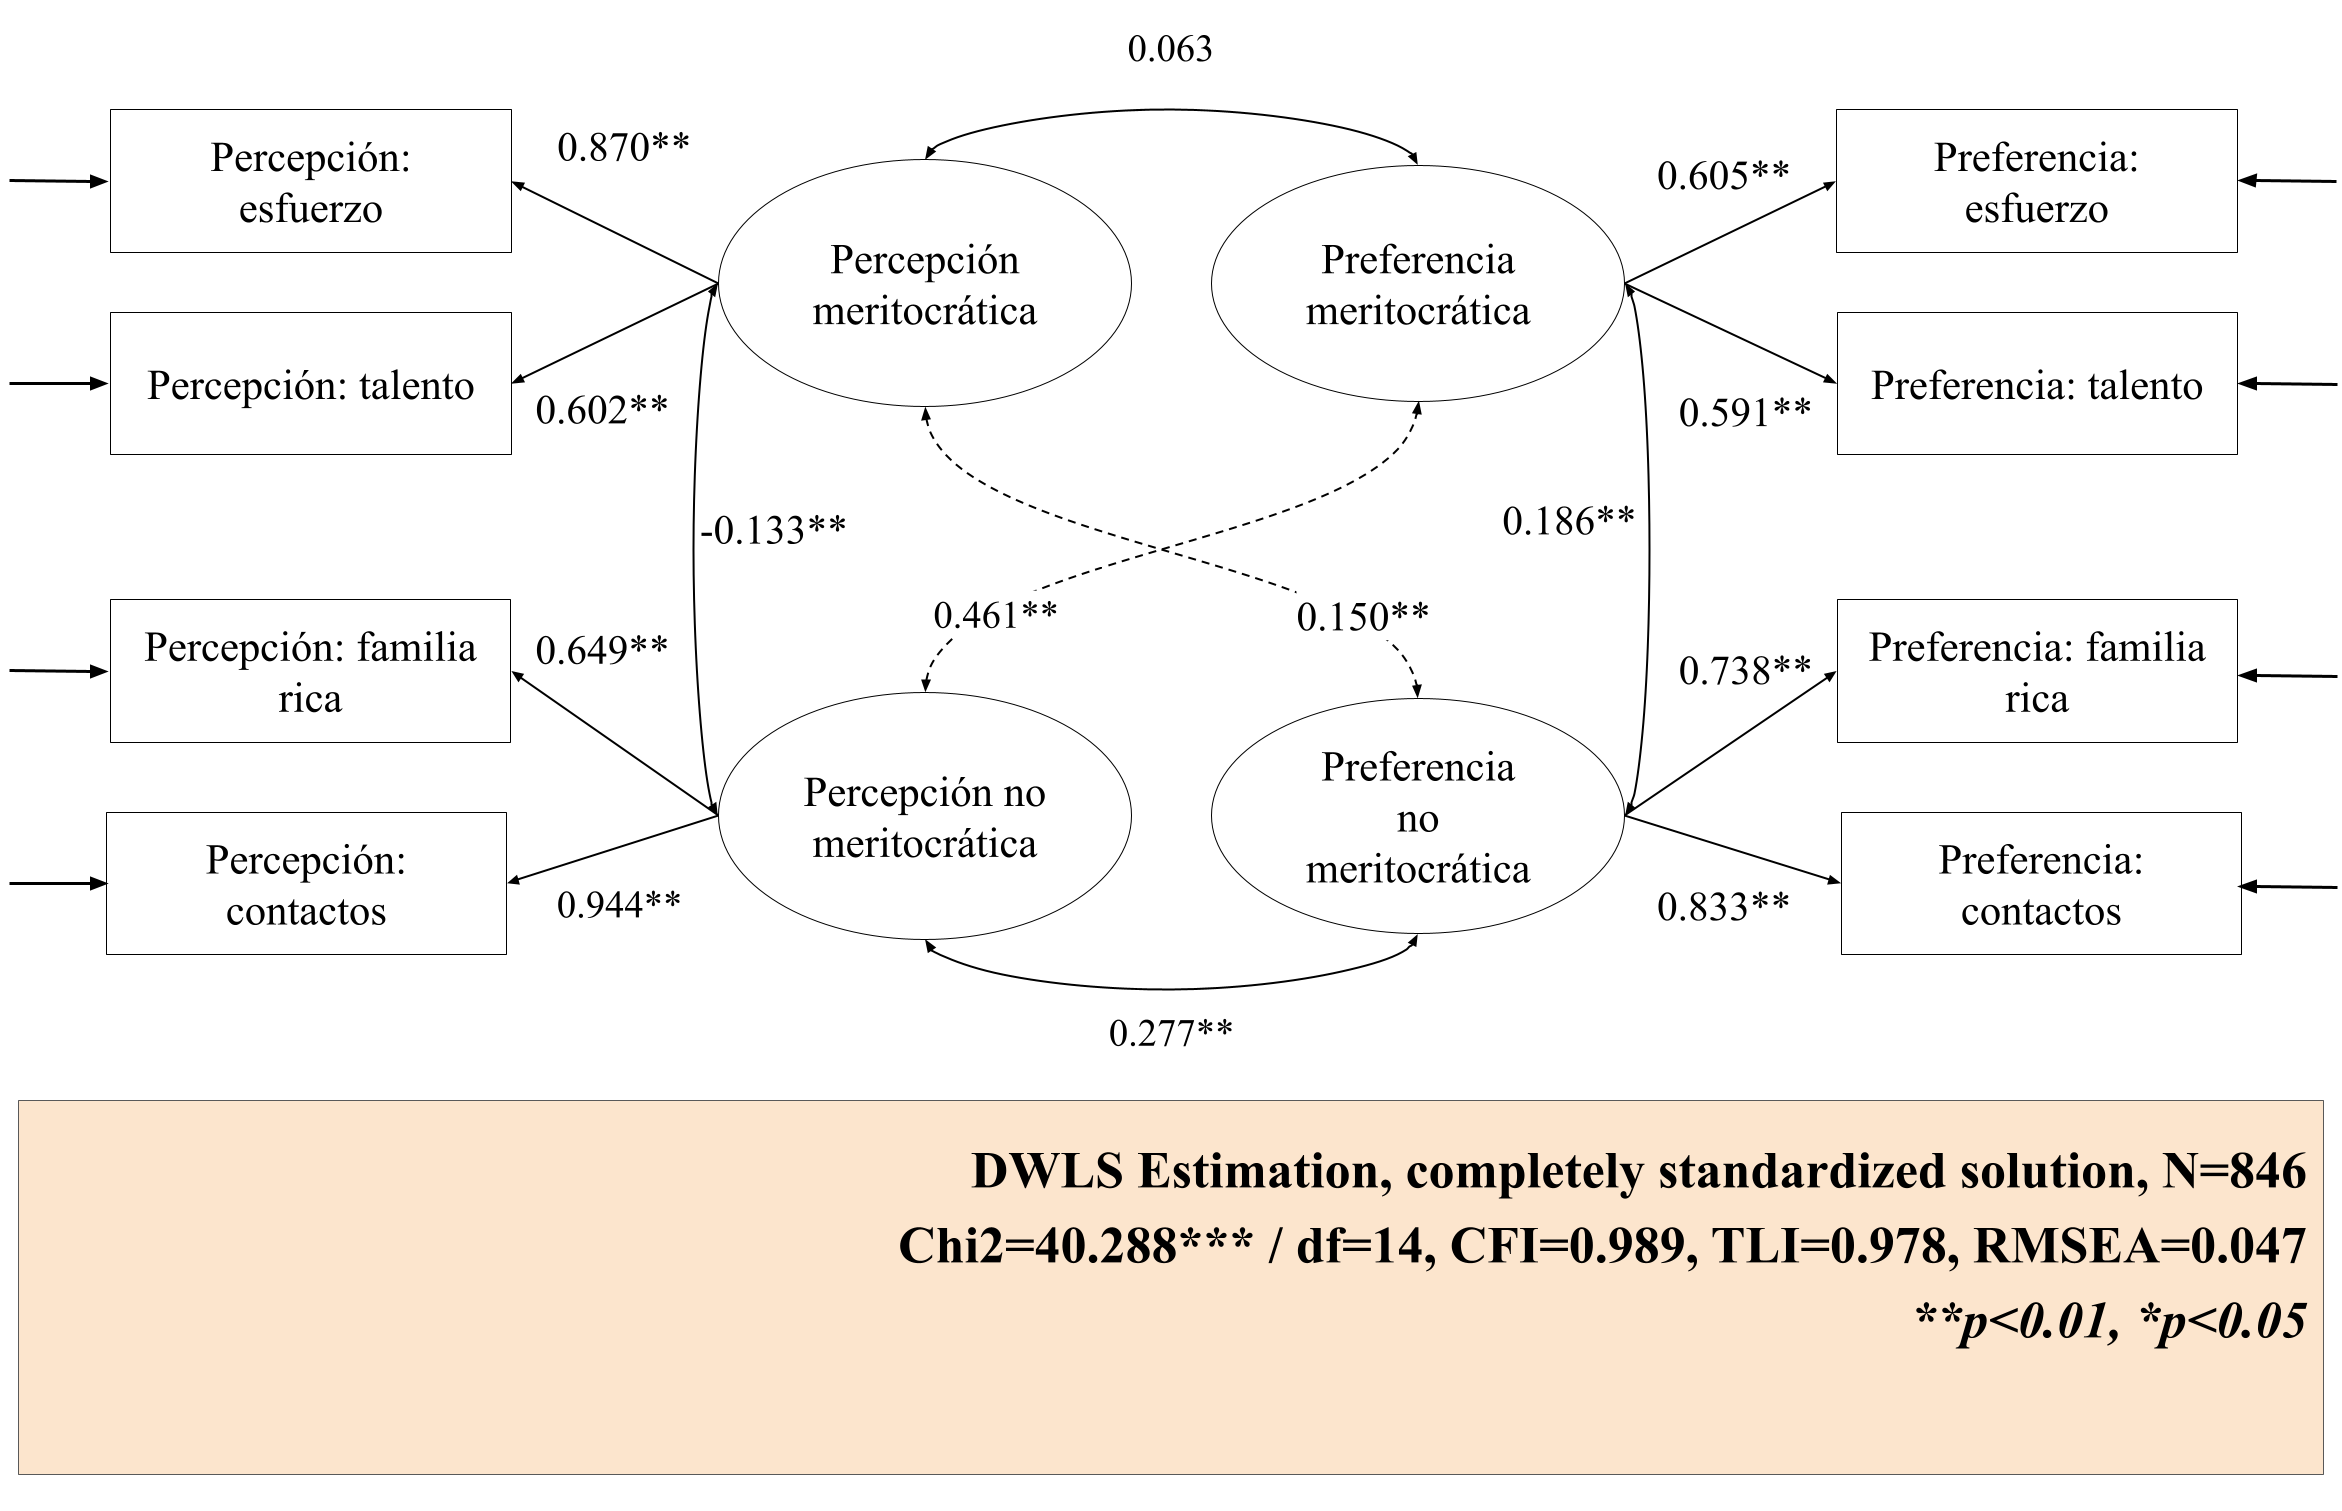
\includegraphics[width=1\textwidth,height=\textheight]{cfa_w1.png}

}

\end{figure}%

En relación con las cargas factoriales, todos los ítems se asocian de
forma positiva y estadísticamente significativa con sus respectivas
dimensiones latentes, y presentan cargas estandarizadas superiores a
0.5, lo que indica una adecuada calidad de la medición
(\citeproc{ref-brown_confirmatory_2015}{Brown, 2015}). Dentro de la
dimensión de percepción meritocrática, el ítem correspondiente al
esfuerzo destaca como el indicador con mayor carga factorial (\(\beta\)
= 0.87, \(p\) \textless{} 0.01), lo que sugiere que este principio
constituye el eje central en las creencias sobre los mecanismos
legítimos del éxito social desde una lógica meritocrática. Por su parte,
en la dimensión de percepción no meritocrática, el ítem referido al uso
de contactos personales presenta la mayor carga (\(\beta\) = 0.944,
\(p\) \textless{} 0.01), posicionándose como el componente más
representativo de esta dimensión. En las dimensiones normativas se
observan patrones similares: en la preferencia por criterios
meritocráticos existe una cierta paridad entre los ítems de esfuerzo y
talento, sin que uno predomine claramente sobre el otro, mientras que en
la preferencia por criterios no meritocráticos nuevamente el uso de
contactos (\(\beta\) = 0.833, \(p\) \textless{} 0.01) emerge como el
criterio normativo más relevante.

Respecto de las correlaciones entre factores, se identifican relaciones
conceptualmente significativas. Por un lado, la percepción de que los
logros sociales se deben a factores meritocráticos se asocia
negativamente con la percepción de que estos se explican por mecanismos
no meritocráticos (\(r\) = -0.133, \(p\)\textless0.01). Por otro lado, y
en contraste con esta lógica excluyente en el plano perceptivo, se
observa una correlación positiva entre las preferencias meritocráticas y
no meritocráticas (\(r\) = 0.186, \(p\)\textless0.01). Este hallazgo
sugiere que, normativamente, ambas lógicas pueden coexistir: los
estudiantes pueden simultáneamente valorar que el esfuerzo o el talento
deban ser recompensados, al mismo tiempo que consideran legítimo que
otros factores, como el origen familiar o los contactos, también
influyan en el acceso a ventajas.

De manera particularmente relevante, se observa una correlación positiva
entre la percepción de mecanismos no meritocráticos y la preferencia por
mecanismos meritocráticos. Específicamente, quienes perciben que el
funcionamiento social se basa en factores no meritocráticos ---como los
contactos personales o el origen familiar--- tienden a manifestar una
mayor preferencia por que elementos meritocráticos, como el esfuerzo y
el talento, sean efectivamente recompensados en la sociedad (\(r\) =
0.461, \(p\) \textless{} 0.01). Este hallazgo sugiere que el
reconocimiento de una realidad social percibida como injusta o alejada
del ideal meritocrático puede reforzar normativamente la adhesión a
principios meritocráticos. En otras palabras, cuanto más se percibe que
operan criterios ajenos al mérito en la distribución de ventajas, mayor
es el deseo de que el mérito ---en particular, el esfuerzo y el
talento--- se convierta en el fundamento legítimo de la recompensa
social.

\begin{figure}

\caption{\label{fig-cfa2}Análisis factorial confirmatorio de Escala de
Meritocracia Ola 2}

\centering{

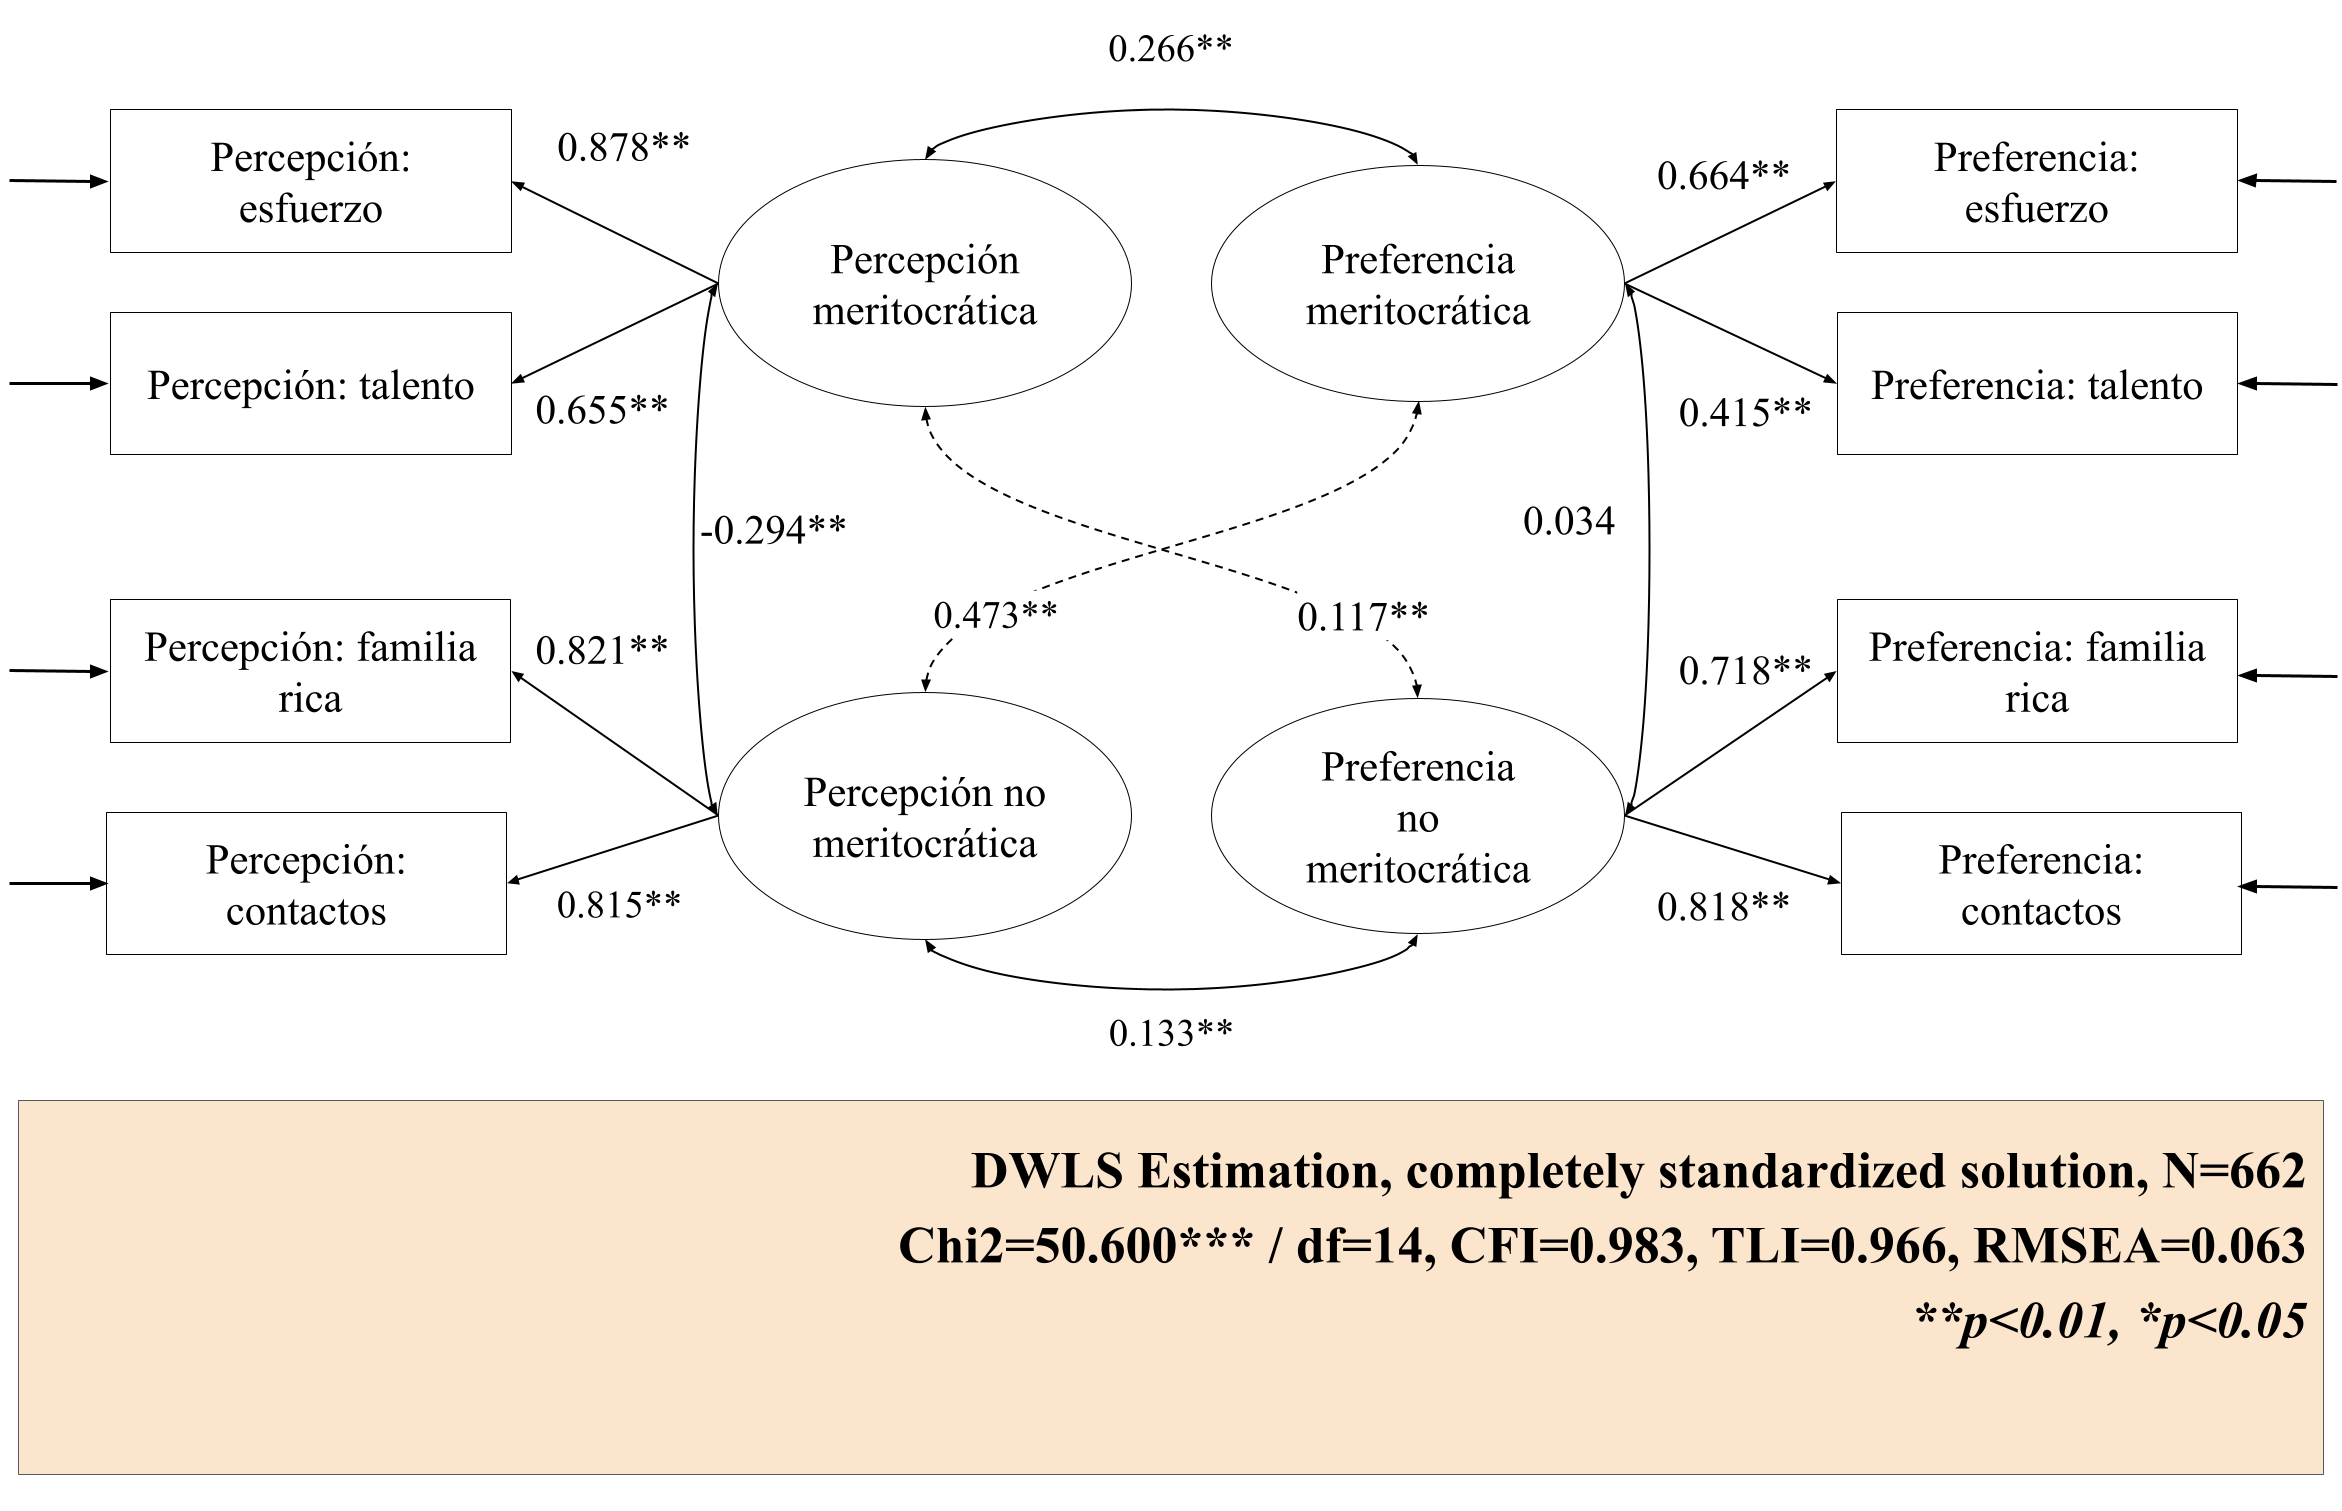
\includegraphics[width=1\textwidth,height=\textheight]{cfa_w2.png}

}

\end{figure}%

En la Figure~\ref{fig-cfa2} se presenta la solución estandarizada del
modelo factorial confirmatorio estimado para la segunda ola del estudio.
Al igual que en la ola anterior, el modelo se encuentra
sobreidentificado, con 14 grados de libertad (\(df\) = 14 \textgreater{}
0), lo que permite una estimación robusta de los parámetros del modelo.

En términos de ajuste global, el estadístico \(\chi^2\) resulta
significativo, lo cual podría sugerir una falta de ajuste. Sin embargo,
como se discutió previamente, este resultado debe ser interpretado con
cautela debido a su sensibilidad al tamaño muestral. En este caso, los
indicadores complementarios ---el índice de ajuste comparativo (CFI) y
el índice de Tucker-Lewis (TLI)--- se sitúan por sobre el umbral de
0.95, lo que indica un buen ajuste relativo del modelo. Por su parte, el
RMSEA alcanza un valor de 0.06, que corresponde a un ajuste razonable
según los criterios establecidos en la literatura especializada
((\citeproc{ref-brown_confirmatory_2015}{Brown, 2015}).

En cuanto a las cargas factoriales, se mantienen los patrones observados
en la ola anterior con algunas variaciones menores. Dentro de la
dimensión de percepción meritocrática, el ítem de esfuerzo continúa
siendo el más relevante, mostrando una carga superior a la del talento.
En la percepción no meritocrática, en cambio, se observa una mayor
paridad entre los indicadores: tanto el ítem de padres ricos como el de
contactos personales contribuyen de manera similar a la dimensión. En lo
que respecta a las preferencias normativas, se confirma nuevamente que
el esfuerzo es el componente con mayor carga factorial dentro de la
dimensión meritocrática, superando al talento. Por su parte, en la
preferencia por criterios no meritocráticos, el ítem que presenta mayor
peso es el de contactos, reafirmando su centralidad en esta dimensión.

Respecto de las correlaciones entre factores, se replican en gran medida
los patrones observados en la primera ola. Se mantiene la correlación
negativa entre percepción meritocrática y percepción no meritocrática,
así como la correlación positiva entre las preferencias por criterios
meritocráticos y no meritocráticos, indicando la persistencia de una
tensión entre representación descriptiva y posicionamiento normativo.
También se conserva la asociación positiva entre percepción no
meritocrática y preferencia por estos mecanismos, lo que refuerza la
hipótesis de legitimación normativa de estructuras no basadas en mérito.

No obstante, un hallazgo distintivo en esta segunda medición es la
emergencia de una correlación positiva y estadísticamente significativa
entre la percepción meritocrática y la preferencia por criterios
meritocráticos, relación que no fue significativa en la ola anterior.
Esto sugiere que, en este momento del estudio, quienes perciben que la
sociedad funciona según principios meritocráticos también tienden a
considerar legítimo que dichos principios guíen la distribución de
recompensas sociales. Esta convergencia entre percepción y preferencia
en el eje meritocrático puede interpretarse como una señal de mayor
coherencia normativa, o bien, como una posible reacción ideológica
frente a cambios contextuales percibidos entre ambas mediciones.

Con todo, los resultados revelan que la escala presenta buenos índices
de ajuste y que sus dimensiones corresponden al modelo multidimensional
propuesto para la población escolar. Se observaron cargas factoriales
altas (\textgreater{} 0.6) para todos los ítems en sus respectivos
factores latentes. Las correlaciones entre factores son consistentes con
las observadas en la población adulta
(\citeproc{ref-castillo_multidimensional_2023}{Castillo et al., 2023}):
la percepción de elementos meritocráticos se asocia negativamente con la
percepción de elementos no meritocráticos, mientras que esta última se
relaciona positivamente con la preferencia por la meritocracia. Estos
hallazgos sugieren que, en una etapa temprana de socialización, los
estudiantes distinguen entre cómo perciben el funcionamiento de
elementos meritocráticos y no meritocráticos y cómo prefieren que estos
operen en la sociedad. Es destacable que una mayor percepción de la no
meritocracia se vincula con una mayor preferencia por la misma, lo que
resalta la importancia de este principio moral en la formación de
valores y actitudes durante los años escolares
(\citeproc{ref-batruch_belief_2022}{Batruch et al., 2022};
\citeproc{ref-darnon_where_2018}{Darnon et al., 2018};
\citeproc{ref-wiederkehr_belief_2015}{Wiederkehr et al., 2015}).

\section{Referencias}\label{referencias}

\phantomsection\label{refs}
\begin{CSLReferences}{1}{0}
\bibitem[\citeproctext]{ref-batruch_belief_2022}
Batruch, A., Jetten, J., Van de Werfhorst, H., Darnon, C., \& Butera, F.
(2022). Belief in {School Meritocracy} and the {Legitimization} of
{Social} and {Income Inequality}. \emph{Social Psychological and
Personality Science}, 194855062211110.
\url{https://doi.org/10.1177/19485506221111017}

\bibitem[\citeproctext]{ref-brown_confirmatory_2015}
Brown, T. A. (2015). \emph{Confirmatory factor analysis for applied
research} (Second edition). New York London: The Guilford Press.

\bibitem[\citeproctext]{ref-castillo_multidimensional_2023}
Castillo, J. C., Iturra, J., Maldonado, L., Atria, J., \& Meneses, F.
(2023). A {Multidimensional Approach} for {Measuring Meritocratic
Beliefs}: {Advantages}, {Limitations} and {Alternatives} to the {ISSP
Social Inequality Survey}. \emph{International Journal of Sociology},
\emph{53}(6), 448--472.
\url{https://doi.org/10.1080/00207659.2023.2274712}

\bibitem[\citeproctext]{ref-chancel_world_2022}
Chancel, L., Piketty, T., Saez, E., \& Zucman, G. (2022). World
inequality report 2022.
https://bibliotecadigital.ccb.org.co/handle/11520/27510.

\bibitem[\citeproctext]{ref-chen_sensitivity_2007}
Chen, F. F. (2007). Sensitivity of {Goodness} of {Fit Indexes} to {Lack}
of {Measurement Invariance}. \emph{Structural Equation Modeling: A
Multidisciplinary Journal}, \emph{14}(3), 464--504.
\url{https://doi.org/10.1080/10705510701301834}

\bibitem[\citeproctext]{ref-corvalan_mercado_2017}
Corvalán, J., Carrasco, A., \& García-Huidobro;J. E. (2017).
\emph{Mercado escolar: {Libertad}, diversidad y desigualdad}. Ediciones
UC.

\bibitem[\citeproctext]{ref-darnon_where_2018}
Darnon, C., Wiederkehr, V., Dompnier, B., \& Martinot, D. (2018).
{``{Where} there is a will, there is a way''}: {Belief} in school
meritocracy and the social-class achievement gap. \emph{British Journal
of Social Psychology}, \emph{57}(1), 250--262.
\url{https://doi.org/10.1111/bjso.12214}

\bibitem[\citeproctext]{ref-davidov_measurement_2014}
Davidov, E., Meuleman, B., Cieciuch, J., Schmidt, P., \& Billiet, J.
(2014). Measurement {Equivalence} in {Cross-National Research}.
\emph{Annual Review of Sociology}, \emph{40}(Volume 40, 2014), 55--75.
\url{https://doi.org/10.1146/annurev-soc-071913-043137}

\bibitem[\citeproctext]{ref-dubet_repensar_2011}
Dubet, F. (2011). \emph{{Repensar la justicia social}} (Sexta
Edici{ó}n). Siglo XXI.

\bibitem[\citeproctext]{ref-kline_principles_2023}
Kline, R. B. (2023). \emph{Principles and {Practice} of {Structural
Equation Modeling}}. Guilford Publications.

\bibitem[\citeproctext]{ref-liu_testing_2017}
Liu, Y., Millsap, R. E., West, S. G., Tein, J.-Y., Tanaka, R., \& Grimm,
K. J. (2017). Testing measurement invariance in longitudinal data with
ordered-categorical measures. \emph{Psychological Methods},
\emph{22}(3), 486--506. \url{https://doi.org/10.1037/met0000075}

\bibitem[\citeproctext]{ref-mijs_paradox_2019}
Mijs, J. (2019). The paradox of inequality: Income inequality and belief
in meritocracy go hand in hand. \emph{Socio-Economic Review},
\emph{19}(1), 7--35. \url{https://doi.org/10.1093/ser/mwy051}

\bibitem[\citeproctext]{ref-wiederkehr_belief_2015}
Wiederkehr, V., Bonnot, V., Krauth-Gruber, S., \& Darnon, C. (2015).
Belief in school meritocracy as a system-justifying tool for low status
students. \emph{Frontiers in Psychology}, \emph{6}.

\bibitem[\citeproctext]{ref-wilson_role_2003a}
Wilson, C. (2003). The {Role} of a {Merit Principle} in {Distributive
Justice}. \emph{The Journal of Ethics}, \emph{7}(3), 277--314.
\url{https://doi.org/10.1023/A:1024667228488}

\bibitem[\citeproctext]{ref-young_rise_1958}
Young, M. (1958). \emph{The rise of the meritocracy}. New Brunswick,
N.J., U.S.A: Transaction Publishers.

\end{CSLReferences}

\pagebreak

\section{Código de R}\label{cuxf3digo-de-r}

\begin{Shaded}
\begin{Highlighting}[]
\FunctionTok{library}\NormalTok{(knitr)}
\NormalTok{knitr}\SpecialCharTok{::}\NormalTok{opts\_chunk}\SpecialCharTok{$}\FunctionTok{set}\NormalTok{(}\AttributeTok{echo =} \ConstantTok{TRUE}\NormalTok{, }\AttributeTok{include =} \ConstantTok{TRUE}\NormalTok{, }\AttributeTok{warning =} \ConstantTok{FALSE}\NormalTok{, }\AttributeTok{message =} \ConstantTok{FALSE}\NormalTok{)}

\NormalTok{table\_format }\OtherTok{\textless{}{-}} \ControlFlowTok{if}\NormalTok{(}\FunctionTok{is\_html\_output}\NormalTok{()) \{}
  \StringTok{"html"}
\NormalTok{\} }\ControlFlowTok{else} \ControlFlowTok{if}\NormalTok{(}\FunctionTok{is\_latex\_output}\NormalTok{()) \{}
  \StringTok{"latex"}
\NormalTok{\}}
\NormalTok{table\_format2 }\OtherTok{\textless{}{-}} \ControlFlowTok{if}\NormalTok{(}\FunctionTok{is\_html\_output}\NormalTok{()) \{}
\NormalTok{  T}
\NormalTok{\} }\ControlFlowTok{else} \ControlFlowTok{if}\NormalTok{(}\FunctionTok{is\_latex\_output}\NormalTok{()) \{}
\NormalTok{  F}
\NormalTok{\}}

\FunctionTok{options}\NormalTok{(}\AttributeTok{kableExtra.html.bsTable =}\NormalTok{ T)}
\FunctionTok{options}\NormalTok{(}\AttributeTok{knitr.kable.NA =} \StringTok{""}\NormalTok{)}
\ControlFlowTok{if}\NormalTok{ (}\SpecialCharTok{!} \FunctionTok{require}\NormalTok{(}\StringTok{"pacman"}\NormalTok{)) }\FunctionTok{install.packages}\NormalTok{(}\StringTok{"pacman"}\NormalTok{)}

\NormalTok{pacman}\SpecialCharTok{::}\FunctionTok{p\_load}\NormalTok{(tidyverse,}
\NormalTok{               sjmisc, }
\NormalTok{               sjPlot,}
\NormalTok{               here,}
\NormalTok{               lavaan,}
\NormalTok{               psych,}
\NormalTok{               corrplot,}
\NormalTok{               ggdist,}
\NormalTok{               patchwork,}
\NormalTok{               sjlabelled,}
\NormalTok{               semTools,}
\NormalTok{               gtools,}
\NormalTok{               RColorBrewer,}
\NormalTok{               skimr,}
\NormalTok{               readxl,}
\NormalTok{               kableExtra)}


\FunctionTok{options}\NormalTok{(}\AttributeTok{scipen=}\DecValTok{999}\NormalTok{)}
\FunctionTok{rm}\NormalTok{(}\AttributeTok{list =} \FunctionTok{ls}\NormalTok{())}
\FunctionTok{load}\NormalTok{(}\AttributeTok{file =} \FunctionTok{here}\NormalTok{(}\StringTok{"output"}\NormalTok{, }\StringTok{"data"}\NormalTok{, }\StringTok{"db\_long\_proc.RData"}\NormalTok{))}


\FunctionTok{names}\NormalTok{(db\_long)}
\FunctionTok{glimpse}\NormalTok{(db\_long)}

\NormalTok{tabla\_merit }\OtherTok{\textless{}{-}} \FunctionTok{data.frame}\NormalTok{(}
  \AttributeTok{Componente =} \FunctionTok{c}\NormalTok{(}\StringTok{"Percepción"}\NormalTok{, }\StringTok{""}\NormalTok{, }\StringTok{""}\NormalTok{, }\StringTok{""}\NormalTok{, }
                 \StringTok{"Preferencia"}\NormalTok{, }\StringTok{""}\NormalTok{, }\StringTok{""}\NormalTok{, }\StringTok{""}\NormalTok{),}
\NormalTok{  Dimensión }\OtherTok{=} \FunctionTok{c}\NormalTok{(}\StringTok{"Meritocrática"}\NormalTok{, }\StringTok{"Meritocrática"}\NormalTok{, }
                \StringTok{"No meritocrática"}\NormalTok{, }\StringTok{"No meritocrática"}\NormalTok{,}
                \StringTok{"Meritocrática"}\NormalTok{, }\StringTok{"Meritocrática"}\NormalTok{, }
                \StringTok{"No meritocrática"}\NormalTok{, }\StringTok{"No meritocrática"}\NormalTok{),}
\NormalTok{  Í}\AttributeTok{tem =} \FunctionTok{c}\NormalTok{(}
    \StringTok{"En Chile, las personas son recompensadas por su esfuerzo."}\NormalTok{,}
    \StringTok{"En Chile, las personas son recompensadas por su inteligencia y habilidades."}\NormalTok{,}
    \StringTok{"En Chile, a quienes tienen padres ricos les va mucho mejor en la vida."}\NormalTok{,}
    \StringTok{"En Chile, a quienes tienen buenos contactos les va mejor en la vida."}\NormalTok{,}
    \StringTok{"Quienes se esfuerzan más deberían recibir mayores recompensas que quienes se esfuerzan menos."}\NormalTok{,}
    \StringTok{"Quienes tienen más talento deberían recibir mayores recompensas que quienes tienen menos talento."}\NormalTok{,}
    \StringTok{"Está bien que a quienes tienen padres ricos les vaya bien en la vida."}\NormalTok{,}
    \StringTok{"Está bien que a quienes tienen buenos contactos les vaya bien en la vida."}
\NormalTok{  )}
\NormalTok{)}

\NormalTok{tabla\_merit }\SpecialCharTok{\%\textgreater{}\%}\NormalTok{ kableExtra}\SpecialCharTok{::}\FunctionTok{kable}\NormalTok{(., }\AttributeTok{format =} \StringTok{"markdown"}\NormalTok{)}

\FunctionTok{theme\_set}\NormalTok{(}\FunctionTok{theme\_ggdist}\NormalTok{())}
\NormalTok{colors }\OtherTok{\textless{}{-}}\NormalTok{ RColorBrewer}\SpecialCharTok{::}\FunctionTok{brewer.pal}\NormalTok{(}\AttributeTok{n =} \DecValTok{4}\NormalTok{, }\AttributeTok{name =} \StringTok{"RdBu"}\NormalTok{)}

\NormalTok{a }\OtherTok{\textless{}{-}}\NormalTok{ db\_long }\SpecialCharTok{\%\textgreater{}\%} 
  \FunctionTok{filter}\NormalTok{(ola }\SpecialCharTok{==} \DecValTok{1}\NormalTok{) }\SpecialCharTok{\%\textgreater{}\%}
  \FunctionTok{select}\NormalTok{(}\FunctionTok{starts\_with}\NormalTok{(}\StringTok{"perc"}\NormalTok{)) }\SpecialCharTok{\%\textgreater{}\%} 
\NormalTok{  sjPlot}\SpecialCharTok{::}\FunctionTok{plot\_likert}\NormalTok{(}\AttributeTok{geom.colors =}\NormalTok{ colors,}
                      \AttributeTok{title =} \FunctionTok{c}\NormalTok{(}\StringTok{"a. Percepciones"}\NormalTok{),}
                      \AttributeTok{geom.size =} \FloatTok{0.8}\NormalTok{,}
                      \AttributeTok{axis.labels =} \FunctionTok{c}\NormalTok{(}\StringTok{"Esfuerzo"}\NormalTok{, }\StringTok{"Talento"}\NormalTok{, }\StringTok{"Padres ricos"}\NormalTok{, }\StringTok{"Contactos"}\NormalTok{),}
                      \AttributeTok{catcount =} \DecValTok{4}\NormalTok{,}
                      \AttributeTok{values  =}  \StringTok{"sum.outside"}\NormalTok{,}
                      \AttributeTok{reverse.colors =}\NormalTok{ F,}
                      \AttributeTok{reverse.scale =}\NormalTok{ T,}
                      \AttributeTok{show.n =} \ConstantTok{FALSE}\NormalTok{,}
                      \AttributeTok{show.prc.sign =}\NormalTok{ T}
\NormalTok{                      ) }\SpecialCharTok{+}
\NormalTok{  ggplot2}\SpecialCharTok{::}\FunctionTok{theme}\NormalTok{(}\AttributeTok{legend.position =} \StringTok{"none"}\NormalTok{)}

\NormalTok{b }\OtherTok{\textless{}{-}}\NormalTok{ db\_long }\SpecialCharTok{\%\textgreater{}\%} 
  \FunctionTok{filter}\NormalTok{(ola }\SpecialCharTok{==} \DecValTok{1}\NormalTok{) }\SpecialCharTok{\%\textgreater{}\%} 
  \FunctionTok{select}\NormalTok{(}\FunctionTok{starts\_with}\NormalTok{(}\StringTok{"pref"}\NormalTok{)) }\SpecialCharTok{\%\textgreater{}\%} 
\NormalTok{  sjPlot}\SpecialCharTok{::}\FunctionTok{plot\_likert}\NormalTok{(}\AttributeTok{geom.colors =}\NormalTok{ colors,}
                      \AttributeTok{title =} \FunctionTok{c}\NormalTok{(}\StringTok{"b. Preferencias"}\NormalTok{),}
                      \AttributeTok{geom.size =} \FloatTok{0.8}\NormalTok{,}
                     \AttributeTok{axis.labels =} \FunctionTok{c}\NormalTok{(}\StringTok{"Esfuerzo"}\NormalTok{, }\StringTok{"Talento"}\NormalTok{, }\StringTok{"Padres ricos"}\NormalTok{, }\StringTok{"Contactos"}\NormalTok{),}
                      \AttributeTok{catcount =} \DecValTok{4}\NormalTok{,}
                      \AttributeTok{values  =}  \StringTok{"sum.outside"}\NormalTok{,}
                      \AttributeTok{reverse.colors =}\NormalTok{ F,}
                      \AttributeTok{reverse.scale =}\NormalTok{ T,}
                      \AttributeTok{show.n =} \ConstantTok{FALSE}\NormalTok{,}
                      \AttributeTok{show.prc.sign =}\NormalTok{ T}
\NormalTok{  ) }\SpecialCharTok{+}
\NormalTok{  ggplot2}\SpecialCharTok{::}\FunctionTok{theme}\NormalTok{(}\AttributeTok{legend.position =} \StringTok{"bottom"}\NormalTok{)}

\NormalTok{likerplot }\OtherTok{\textless{}{-}}\NormalTok{ a }\SpecialCharTok{/}\NormalTok{ b }\SpecialCharTok{+} \FunctionTok{plot\_annotation}\NormalTok{(}\AttributeTok{caption =} \FunctionTok{paste0}\NormalTok{(}\StringTok{"Fuente: Elaboración propia en base a Encuesta Panel EDUMER Ola 1"}\NormalTok{,}\StringTok{" (n = "}\NormalTok{,}\FunctionTok{dim}\NormalTok{(db\_long[db\_long}\SpecialCharTok{$}\NormalTok{ola}\SpecialCharTok{==}\DecValTok{1}\NormalTok{,])[}\DecValTok{1}\NormalTok{],}\StringTok{")"}
\NormalTok{))}

\NormalTok{likerplot}


\NormalTok{M }\OtherTok{\textless{}{-}}\NormalTok{ psych}\SpecialCharTok{::}\FunctionTok{polychoric}\NormalTok{(db\_long[db\_long}\SpecialCharTok{$}\NormalTok{ola}\SpecialCharTok{==}\DecValTok{1}\NormalTok{,][}\FunctionTok{c}\NormalTok{(}\DecValTok{4}\SpecialCharTok{:}\DecValTok{11}\NormalTok{)])}

\FunctionTok{diag}\NormalTok{(M}\SpecialCharTok{$}\NormalTok{rho) }\OtherTok{\textless{}{-}} \ConstantTok{NA}

\FunctionTok{rownames}\NormalTok{(M}\SpecialCharTok{$}\NormalTok{rho) }\OtherTok{\textless{}{-}} \FunctionTok{c}\NormalTok{(}\StringTok{"A. Percepción Esfuerzo"}\NormalTok{,}
                     \StringTok{"B. Percepción Talento"}\NormalTok{,}
                     \StringTok{"C. Percepción Padres Ricos"}\NormalTok{,}
                     \StringTok{"D. Percepción Contactos"}\NormalTok{,}
                     \StringTok{"E. Preferencia Esfuerzo"}\NormalTok{,}
                     \StringTok{"F. Preferencia Talento"}\NormalTok{,}
                     \StringTok{"G. Preferencia Padres Ricos"}\NormalTok{,}
                     \StringTok{"H. Preferencia Contactos"}\NormalTok{)}

\CommentTok{\#set Column names of the matrix}
\FunctionTok{colnames}\NormalTok{(M}\SpecialCharTok{$}\NormalTok{rho) }\OtherTok{\textless{}{-}}\FunctionTok{c}\NormalTok{(}\StringTok{"(A)"}\NormalTok{, }\StringTok{"(B)"}\NormalTok{,}\StringTok{"(C)"}\NormalTok{,}\StringTok{"(D)"}\NormalTok{,}\StringTok{"(E)"}\NormalTok{,}\StringTok{"(F)"}\NormalTok{,}\StringTok{"(G)"}\NormalTok{,}
                    \StringTok{"(H)"}\NormalTok{)}

\NormalTok{testp }\OtherTok{\textless{}{-}} \FunctionTok{cor.mtest}\NormalTok{(M}\SpecialCharTok{$}\NormalTok{rho, }\AttributeTok{conf.level =} \FloatTok{0.95}\NormalTok{)}


\NormalTok{df }\OtherTok{\textless{}{-}} \FunctionTok{as.data.frame}\NormalTok{(M}\SpecialCharTok{$}\NormalTok{rho)}
 
\NormalTok{mat\_cor }\OtherTok{\textless{}{-}} \FunctionTok{as.matrix}\NormalTok{(df)}


\NormalTok{p\_stars }\OtherTok{\textless{}{-}}\NormalTok{ gtools}\SpecialCharTok{::}\FunctionTok{stars.pval}\NormalTok{(testp}\SpecialCharTok{$}\NormalTok{p)}

\NormalTok{mat\_cor\_rounded }\OtherTok{\textless{}{-}} \FunctionTok{round}\NormalTok{(mat\_cor, }\DecValTok{2}\NormalTok{)}
\NormalTok{mat\_cor\_char }\OtherTok{\textless{}{-}} \FunctionTok{format}\NormalTok{(mat\_cor\_rounded, }\AttributeTok{nsmall =} \DecValTok{2}\NormalTok{)}

\NormalTok{cor\_with\_stars }\OtherTok{\textless{}{-}} \FunctionTok{ifelse}\NormalTok{(}\FunctionTok{is.na}\NormalTok{(mat\_cor\_char), }\StringTok{""}\NormalTok{, }
                         \FunctionTok{paste0}\NormalTok{(mat\_cor\_char, p\_stars))}

\NormalTok{cor\_with\_stars[}\FunctionTok{upper.tri}\NormalTok{(cor\_with\_stars, }\AttributeTok{diag =} \ConstantTok{TRUE}\NormalTok{)] }\OtherTok{\textless{}{-}} \ConstantTok{NA}


\NormalTok{cor\_with\_stars }\SpecialCharTok{\%\textgreater{}\%} 
\NormalTok{  kableExtra}\SpecialCharTok{::}\FunctionTok{kable}\NormalTok{(., }\AttributeTok{format =} \StringTok{"markdown"}\NormalTok{) }\SpecialCharTok{\%\textgreater{}\%} 
\NormalTok{  kableExtra}\SpecialCharTok{::}\FunctionTok{add\_footnote}\NormalTok{(}\AttributeTok{label =} \StringTok{"**p\textless{}0.01, *p\textless{}0.5"}\NormalTok{, }\AttributeTok{notation =} \StringTok{"none"}\NormalTok{)}



\CommentTok{\# model}
\NormalTok{model\_cfa }\OtherTok{\textless{}{-}} \StringTok{\textquotesingle{}}
\StringTok{  perc\_merit = \textasciitilde{} perc\_effort + perc\_talent}
\StringTok{  perc\_nmerit = \textasciitilde{} perc\_rich\_parents + perc\_contact}
\StringTok{  pref\_merit = \textasciitilde{} pref\_effort + pref\_talent}
\StringTok{  pref\_nmerit = \textasciitilde{} pref\_rich\_parents + pref\_contact}
\StringTok{  \textquotesingle{}}

\CommentTok{\# estimation for each order set}

\NormalTok{m1\_cfa }\OtherTok{\textless{}{-}} \FunctionTok{cfa}\NormalTok{(}\AttributeTok{model =}\NormalTok{ model\_cfa, }
              \AttributeTok{data =} \FunctionTok{subset}\NormalTok{(db\_long, ola }\SpecialCharTok{==} \DecValTok{1}\NormalTok{),}
              \AttributeTok{estimator =} \StringTok{"DWLS"}\NormalTok{,}
              \AttributeTok{ordered =}\NormalTok{ T,}
              \AttributeTok{std.lv =}\NormalTok{ F) }

\NormalTok{m2\_cfa }\OtherTok{\textless{}{-}} \FunctionTok{cfa}\NormalTok{(}\AttributeTok{model =}\NormalTok{ model\_cfa, }
              \AttributeTok{data =} \FunctionTok{subset}\NormalTok{(db\_long, ola }\SpecialCharTok{==} \DecValTok{2}\NormalTok{), }
              \AttributeTok{estimator =} \StringTok{"DWLS"}\NormalTok{,}
              \AttributeTok{ordered =}\NormalTok{ T,}
              \AttributeTok{std.lv =}\NormalTok{ F)}

\NormalTok{knitr}\SpecialCharTok{::}\FunctionTok{include\_graphics}\NormalTok{(}\AttributeTok{path =} \FunctionTok{here}\NormalTok{(}\StringTok{"sem/cfa\_w1.png"}\NormalTok{))}
\NormalTok{knitr}\SpecialCharTok{::}\FunctionTok{include\_graphics}\NormalTok{(}\AttributeTok{path =} \FunctionTok{here}\NormalTok{(}\StringTok{"sem/cfa\_w2.png"}\NormalTok{))}
\end{Highlighting}
\end{Shaded}




\end{document}
